%%
%% JMU Honors College Format Style
%%  
%% This file was crafted originally
%% by Daniel O. Awduche, Christopher A. St. Jean and Muhammad Abdulla
%% at George Mason University.
%% The file was modified for the JMU honors college format
%% by Kevin Molloy.
%%
%% Notes on usage can be found in the accompanying USAGE_NOTES.txt file.
%%
%%**********************************************************************
%% Legal Notice:
%% This code is offered as-is without any warranty either
%% expressed or implied; without even the implied warranty of
%% MERCHANTABILITY or FITNESS FOR A PARTICULAR PURPOSE!
%% User assumes all risk.
%% In no event shall any contributor to this code be liable for any damages
%% or losses, including, but not limited to, incidental, consequential, or
%% any other damages, resulting from the use or misuse of any information
%% contained here.
%%**********************************************************************
%%

\documentclass[12 pt]{report}

%%  The file ``thesis.sty''  is the JMU honors college latex style file and
%%   should be placed in the same directory as your LaTeX files
\usepackage{ctable}

\usepackage{thesis}

%%
%% other packages that need to be loaded
%%
\usepackage{graphicx}                    %   for imported graphics
\usepackage{amsmath}                     %%
\usepackage{amsfonts}                    %%  for AMS mathematics
\usepackage{amssymb}                     %%
\usepackage{amsthm}                      %%
\usepackage[normalem]{ulem}              %   a nice standard underline package
\usepackage[noadjust,verbose,sort]{cite} %   arranges reference citations neatly
\usepackage{setspace}                    %   for line spacing commands
\usepackage{times}

%\setromanfont{Times New Roman}

\graphicspath{{./figs/}}  %% Where the figures live

\beforedoc

\begin{document}

%% In this section, all of the user-specific fields to be used in the
%% title pages are set
\title{First line of the title\\
            second line of the title}
\onelinetitle{The complete title is to be repeated here without any line
        breaks for the second page and for the abstract page}
\author{Student}
\degree{Bachelor of Science}
\doctype{Thesis}
\dept{Computer Science}
\discipline{Computer Science}
\submitdate{June 2020}

\degreeyear{}

% Note: semester name should be written in its full-form. For example, Fall Semester, not just Fall.
\degreesemester{Semester}

\advisor{Dee A.B Weikle, Ph.D} 
\advisorrank{Associate Professor}
\advisordept{Computer Science}

\firstmember{Michael S. Kirkpatrick, Ph.D}
\firstmemberRole{Reader}
\firstrank{Associate Professor}
\firstdept{Computer Science}


\secondmember{Christopher S. Mayfield, Ph.D}
\secondmemberRole{Reader}
\secondrank{Associate Professor}
\seconddept{Computer Science}


\thirdmember{Angela W. Webb, Ph.D}
\thirdmemberRole{Reader}
\thirdrank{Assistant Professor}
\thirddept{MSME}

\presentLocation{ISAT/CS Room 246}
\presentDate{April 20, 2020}

\deanHonorsCollege{Bradley R. Newcomer, Ph.D.}

%%
%% Introductory pages
%%

% Note: The signature sheet is set according to the requirements of the Volgenau School of
% Information Technology and Engineering. If your college/school requirement is different,
% please make appropriate changes in the "signaturepage" section of gmudissertation.sty file.

\signaturepage

%\titlepage

% copyright technically optional but should be included in to avoid potential pagination problems
\copyrightpage

%%
%% Dedication page
%%

\dedicationpage

\noindent I dedicate this dissertation to ...
I dedicate this dissertation to ...
I dedicate this dissertation to ...
I dedicate this dissertation to ...
I dedicate this dissertation to ...
I dedicate this dissertation to ...
I dedicate this dissertation to ...



\noindent I would like to thank the following people who made this possible ...
I would like to thank the following people who made this possible ...

%%
%% Table of contents, list of tables, and lists of figures
%%

\tableofcontents

\listoftables

\listoffigures

%%
%% Acknowledgements
%%

\acknowledgementspage

%%
%% Abstract
%%
\abstractpage

% The first page of the abstract https://wiki.cs.jmu.edu/department/honors_capstone/start

%% Be sure to leave a line of whitespace immediately before this line!!!!!
%% (If this comment segment runs together with the preceeding text, you might
%%  see the second page of the abstract numbered "0".)
%%
%% If the abstract is more than one page, then place this line PRECISELY
%% at the page break; otherwise, comment it out.  (See note about this line
%% in the usage notes.)
%%
%\abstractmultiplepage
%
%The second page of the abstract
%
%
%
%%
%%  the main body of the dissertation
%%
\startofchapters

%% include the chapters one by one (or paste the chapter text in directly if desired)

%% This file represents a sample first chapter of the main body of the dissertation
%%

% A first, optional argument in [ ] is the title as displayed in the table of contents
% The second argument is the title as displayed here.  Use \\ as appropriate in
%   this title to get desired line breaks
\chapter[Introduction]{Introduction}

\section{Background}
\section{Previous Work} % Literature Review?

Prior work in this field did xyz, and we need to write a line long enough so that we can see both the left and right hand margins.

Lorem ipsum, dolor sit amet consectetur adipisicing elit. Iure quod voluptatum cumque architecto tempora nobis dolorum vitae. Eius ipsa libero, \cite{matt_eg_1} rerum nesciunt voluptatum rem quis quos animi et sunt nihil.
Lorem ipsum, dolor sit amet consectetur adipisicing elit. Iure quod voluptatum cumque architecto tempora nobis dolorum vitae. Eius ipsa libero, rerum nesciunt voluptatum rem quis quos animi et sunt nihil.
Lorem ipsum, dolor sit amet consectetur adipisicing elit. Iure quod voluptatum cumque architecto tempora nobis dolorum vitae. Eius ipsa libero, rerum nesciunt voluptatum rem quis quos animi et sunt nihil.


Lorem ipsum, dolor sit amet consectetur adipisicing elit. Iure quod voluptatum cumque architecto tempora nobis dolorum vitae. Eius ipsa libero, rerum nesciunt voluptatum rem quis quos animi et sunt nihil.
\begin{enumerate}
  \item item 1
  
  \item item 2
  
  \item item 3
  
  \item item 4 
\end{enumerate}


\begin{figure}
  \centering
  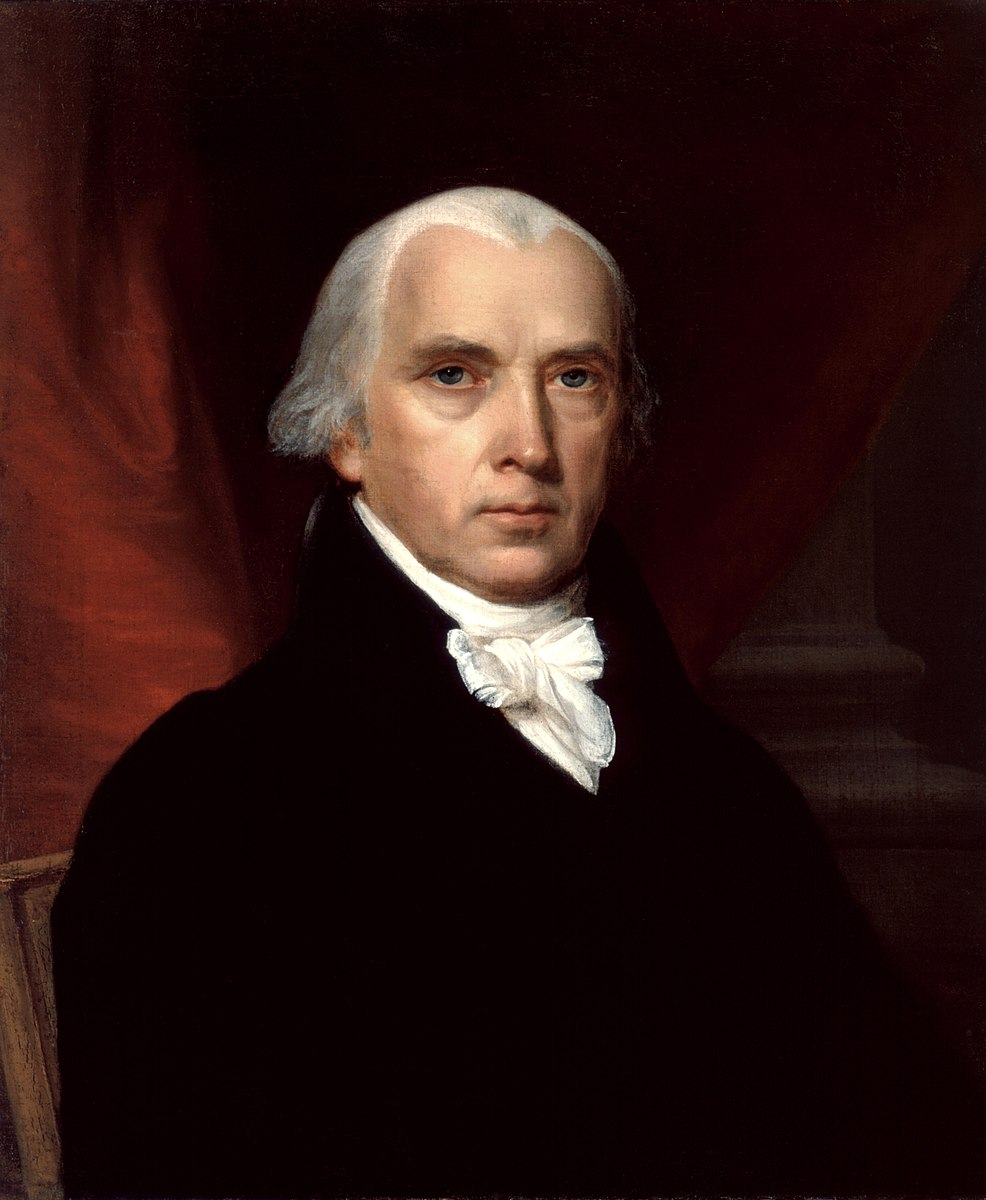
\includegraphics[scale=0.2]{figJamesMadison}
  \caption[An appropriate historical figure]{An appropriate historical figure.}

  % If you need more separation space between this figure and either another figure, or between
  %     the figure and the text, you can add figSpace as shown here.
  \figSpace
\end{figure}

\newpage

\subsection{A Subsection}

Important previous work was also provided by \cite{Shannon49}.  Here is a numbered equation:
\begin{equation}
    f_X(x) = \lambda e^{-\lambda x} u(x).
\end{equation}

Lorem ipsum, dolor sit amet consectetur adipisicing elit. Iure quod voluptatum cumque architecto tempora nobis dolorum vitae. Eius ipsa libero, rerum nesciunt voluptatum rem quis quos animi et sunt nihil.

\subsubsection{A subsubsection}

Lorem ipsum, dolor sit amet consectetur adipisicing elit. Iure quod voluptatum cumque architecto tempora nobis dolorum vitae. Eius ipsa libero, rerum nesciunt voluptatum rem quis quos animi et sunt nihil.

\paragraph{A paragraph}

Lorem ipsum, dolor sit amet consectetur adipisicing elit. Iure quod voluptatum cumque architecto tempora nobis dolorum vitae. Eius ipsa libero, rerum nesciunt voluptatum rem quis quos animi et sunt nihil.

\subparagraph{A subparagraph}

Lorem ipsum, dolor sit amet consectetur adipisicing elit. Iure quod voluptatum cumque architecto tempora nobis dolorum vitae. Eius ipsa libero, rerum nesciunt voluptatum rem quis quos animi et sunt nihil.



\begin{table}
  \centering
  \caption{A table}
  % Tabular environment goes AFTER the caption!
  \begin{tabular}{|c|c|c|}
    % after \\: \hline or \cline{col1-col2} \cline{col3-col4} ...
    \hline
    A & B & C \\\hline
    D & E & F \\\hline
    G & H & I \\
    \hline
  \end{tabular}

  % This adds separation space between this table and either another table, or between
  %     the table and the text.
  \tableSpace
\end{table}


\begin{table}
  \centering
  \caption{Another table}
  % Tabular environment goes AFTER the caption!
  \begin{tabular}{|c|c|c|}
    % after \\: \hline or \cline{col1-col2} \cline{col3-col4} ...
    \hline
    1 & 2 & 3 \\\hline
    4 & 5 & 6 \\\hline
    7 & 8 & 9 \\
    \hline
  \end{tabular}

  % This adds separation space between this table and either another table, or between
  %     the table and the text.
  \tableSpace
\end{table}

%\include{chapterTwo}
%\include{chapterThree}
%\include{chapterFour}

%% Note: appendix is now put before bibliography.
%% include the following directives if there are any appendices
\appendix
\appendixeqnumbering
\include{Appendix}

%%
%%  bibliography
%%

%% list all of the BibTeX files here for the WinEdt project (if applicable)
%GATHER{bibfile.bib}

%% any bibliography style can be used, but IEEEtran.bst is ideally suited to
%% electrical engineering references

\bibliographystyle{IEEEtran}
\bibliography{IEEEfull,bibfile}

%%
%% curriculum vitae
%%
%\cvpage

%\noindent Include your \emph{curriculum vitae} here detailing your background,
%education, and professional experience.


\end{document}
